En el marco de trabajo se ha optado por investigar en base al análisis criminal de redes delictivas en el Ministerio Público Fiscal del Chubut ~\cite{ref_article30}, perteneciente al Poder Judicial de la provincia.

Coirón, es el sistema informático que colabora con la administración del flujo de casos ingresados al Ministerio Público Fiscal del Chubut.

Es una herramienta que permite registrar, comunicar y gestionar las actividades, trámites y actuaciones que se realizan para un caso penal, desde la denuncia hasta su finalización.

Como herramienta de registro construye una base de datos con el historial de cada caso, así como de las personas involucradas y de los responsables de la gestión en cada oficina.
Como herramienta de comunicación, agrupa la información, entrecruza las relaciones, identifica pertenencias y vinculaciones entre casos, personas, sus antecedentes y sus lazos.

Como herramienta de gestión administra el flujo de casos y el trabajo de los integrantes de las oficinas responsables de los mismos. Permite planificar, organizar, coordinar y controlar el flujo de trabajo afín a cada caso y la sumatoria de ellos.
Ha sido desarrollado a medida de las necesidades del Ministerio Público Fiscal del Chubut, tomando como base el Código Procesal Penal vigente en el Chubut y adaptado a los lineamientos estratégicos de diseño y gestión de Oficinas Fiscales definidos por la Procuración General.

Su progreso, mantenimiento y mejora continua está a cargo de un Equipo de Desarrollo del Departamento de Informática del Área de Planificación y Control de Gestión de la Procuración General, del cual formo parte.
\todo{Hablo en singular? plural?}

Una vez registrada toda la información relacionada a un hecho, y con ayuda de herramientas y vinculaciones con otros sistemas, se pueden obtener salidas que permiten llevar adelante la
investigación de un caso o de un conjunto de hechos con características comunes.

Actualmente nos encontramos trabajando en la incorporación de herramientas de visualización de información que permitirán ver en modo gráfico lo que hoy se muestra en grillas, y listados, potenciando el análisis que realizarán luego los especialistas.

Un medio de enfrentar, "a través del análisis criminal, la persecución penal de sujetos prolíficos es el perfilamiento relacional entre ellos, a través de la realización de vinculación de compañeros de delitos y de redes sociales; a fin de identificar si forman parte de una banda o alguna organización criminal mayor o de un fenómeno delictual más extenso"~\cite{ref_article31}.

Los analistas de redes sociales utilizan dos tipos de herramientas matemáticas para representar información sobre los patrones de relaciones entre actores sociales: matrices y grafos. Estos últimos son de gran ayuda visual cuando se trabaja con una gran cantidad de registros.

Existen muchas variaciones en los grafos, pero todos ellos comparten la característica común del uso de un círculo etiquetado para cada actor en la población que describimos y segmentos de línea entre pares de actores para representar el hecho que existe un vínculo entre ellos.

Se denomina "Grupo de Pertenencia" en el Sistema Coirón a la relación directa que existe entre un individuo dentro del universo de personas cargadas como actores de delitos (roles: denunciado, sospechoso o imputado) y otros individuos del mismo universo, con los cuales existan uno o más casos penales en común.

Crear un módulo de software "Red de Grupos de Pertenencia" donde se muestre gráficamente las relaciones entre las personas involucradas en los casos penales es el objetivo principal de esta investigación. No sólo enfocarse en el grupo de pertenencia de una persona en particular, sino que mediante una visualización y con diversos filtros de búsqueda se logre mostrar gráficamente las relaciones entre un determinado grupo de personas y de esta manera poder inferir la conformación de posibles bandas delictivas.

La idea central es reflejar de manera gráfica, mediante un Grafo, los grupos de pertenencia. Dentro del mismo se le llamará nodo a cada círculo, y representa a una persona (con los roles ya mencionados: imputado, sospechoso o denunciado) involucrada en dos o más casos penales. Existe un gran cúmulo de personas en el sistema con sólo un caso con rol de denunciado, por esa razón se los excluye del universo a analizar, no obstante podrían ser parte del dataset a visualizar si alguno/s de ellos se encuentran relacionados con otros nodos del primer grupo. El tamaño del nodo posee una relación directa con la cantidad de casos penales en los que se encuentre involucrada la persona. Cuanto mayor sea el tamaño del nodo en más cantidad de casos penales estará involucrado.

Los segmentos de líneas entre pares de nodos, vinculan a las personas entre sí y representan el o los casos que tienen en común. El grosor de la vinculación será directamente proporcional a la cantidad de casos en común entre un par de personas. 

Hay nodos que se encontrarán aislados en el grafo, esto no significa que no estén involucrados en casos, sino que quizás no existan relaciones para el filtro de búsqueda que se utilice en esa vista en particular.

Supongamos que una persona "A" se encuentra asociada a 6 casos penales y una persona "B" a 3 casos. Agreguemos que ambas se encuentran relacionadas entre sí, por estar en 2 casos en común (caso 1 y 2). Una representación gráfica de dicha situación se muestra a continuación en la Figura \ref{fig:grafode2}. 

\todo{Explicar ejemplos del grafo}

\begin{figure}
	\centering
	\tikzstyle{nodoA}= [circle,fill=blue!25,minimum size=40pt]
	\tikzstyle{nodoB}=[circle,fill=blue!25,minimum size=20pt]
	\begin{center}
		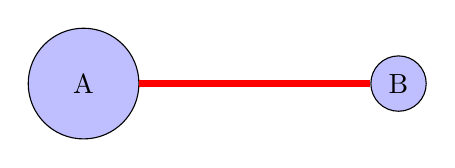
\begin{tikzpicture}[scale=1.0]
			\node[nodoA][draw] (1) at (0,5) {A};
			\node[nodoB][draw] (2) at (4,5) {B};
			%
			\draw [line width=0.8mm, red ] (1) -- (2);
		\end{tikzpicture}
	\end{center}
	\caption{Ejemplo de relación entre dos personas.} 
	\label{fig:grafode2}
\end{figure}
